\documentclass[12pt]{article}
% Set target color model to RGB
\usepackage[a4paper, inner=2.0cm,outer=2.0cm,top=2.0cm,bottom=2.0cm]{geometry}
%\usepackage{setspace}
\usepackage[rgb]{xcolor}
\usepackage{verbatim}
\usepackage{subcaption}
\usepackage{graphicx}
\usepackage{fancyhdr}
\usepackage{xurl}
\usepackage{lipsum}
\usepackage[colorlinks=true, urlcolor=blue,  linkcolor=blue, citecolor=blue]{hyperref}

\usepackage{fontspec}
\setmainfont{Times New Roman}
\usepackage[francais]{babel}

\newcommand{\homework}[5]{
   \pagestyle{myheadings}
   \thispagestyle{plain}
   \newpage
   \setcounter{page}{1}
   \noindent
   \begin{center}
   \framebox{
      \vbox{\vspace{2mm}
    \hbox to 6.28in { {\bf #3 \hfill {\small (#2)}} }
       \vspace{6mm}
       \hbox to 6.28in { {\Large \hfill #1 \hfill} }
       \vspace{6mm}
       \hbox to 6.28in { {\it Etudiant: {\rm #4}, \hfill matricule: {\rm #5}} }
      \vspace{2mm}}
   }
   \end{center}
   \markboth{#5 -- #1}{#5 -- #1}
   \vspace*{4mm}
}

\newcommand{\codeword}[1]{%
\texttt{\textcolor{blue}{#1}}%
}
\newcommand{\weblink}[1]{%
\texttt{\textcolor{blue}{\underline{#1}}}%
}

\newtoks\student
\newtoks\studentid
\newtoks\course
\newtoks\duedate
\newtoks\assignmentname
\newtoks\pdftitle

\student{Etudiant TUTEST}
\studentid{17000000}
\course{Communication \& Leadership 2020}
\duedate{30/03/20}
\assignmentname{Rapport Activité \#1}
\pdftitle{HEC-BA2P-CL-Activite1}

\hypersetup{
pdfauthor={\the\student},
pdftitle={\the\pdftitle},
}

\linespread{1.1}
\setlength\parindent{0pt} % sets indent to zero
\setlength{\parskip}{\baselineskip} % changes vertical space between paragraphs

\begin{document}
\homework{\the\assignmentname}{Due: \the\duedate}{\the\course}{\the\student}{\the\studentid}

\begin{center}
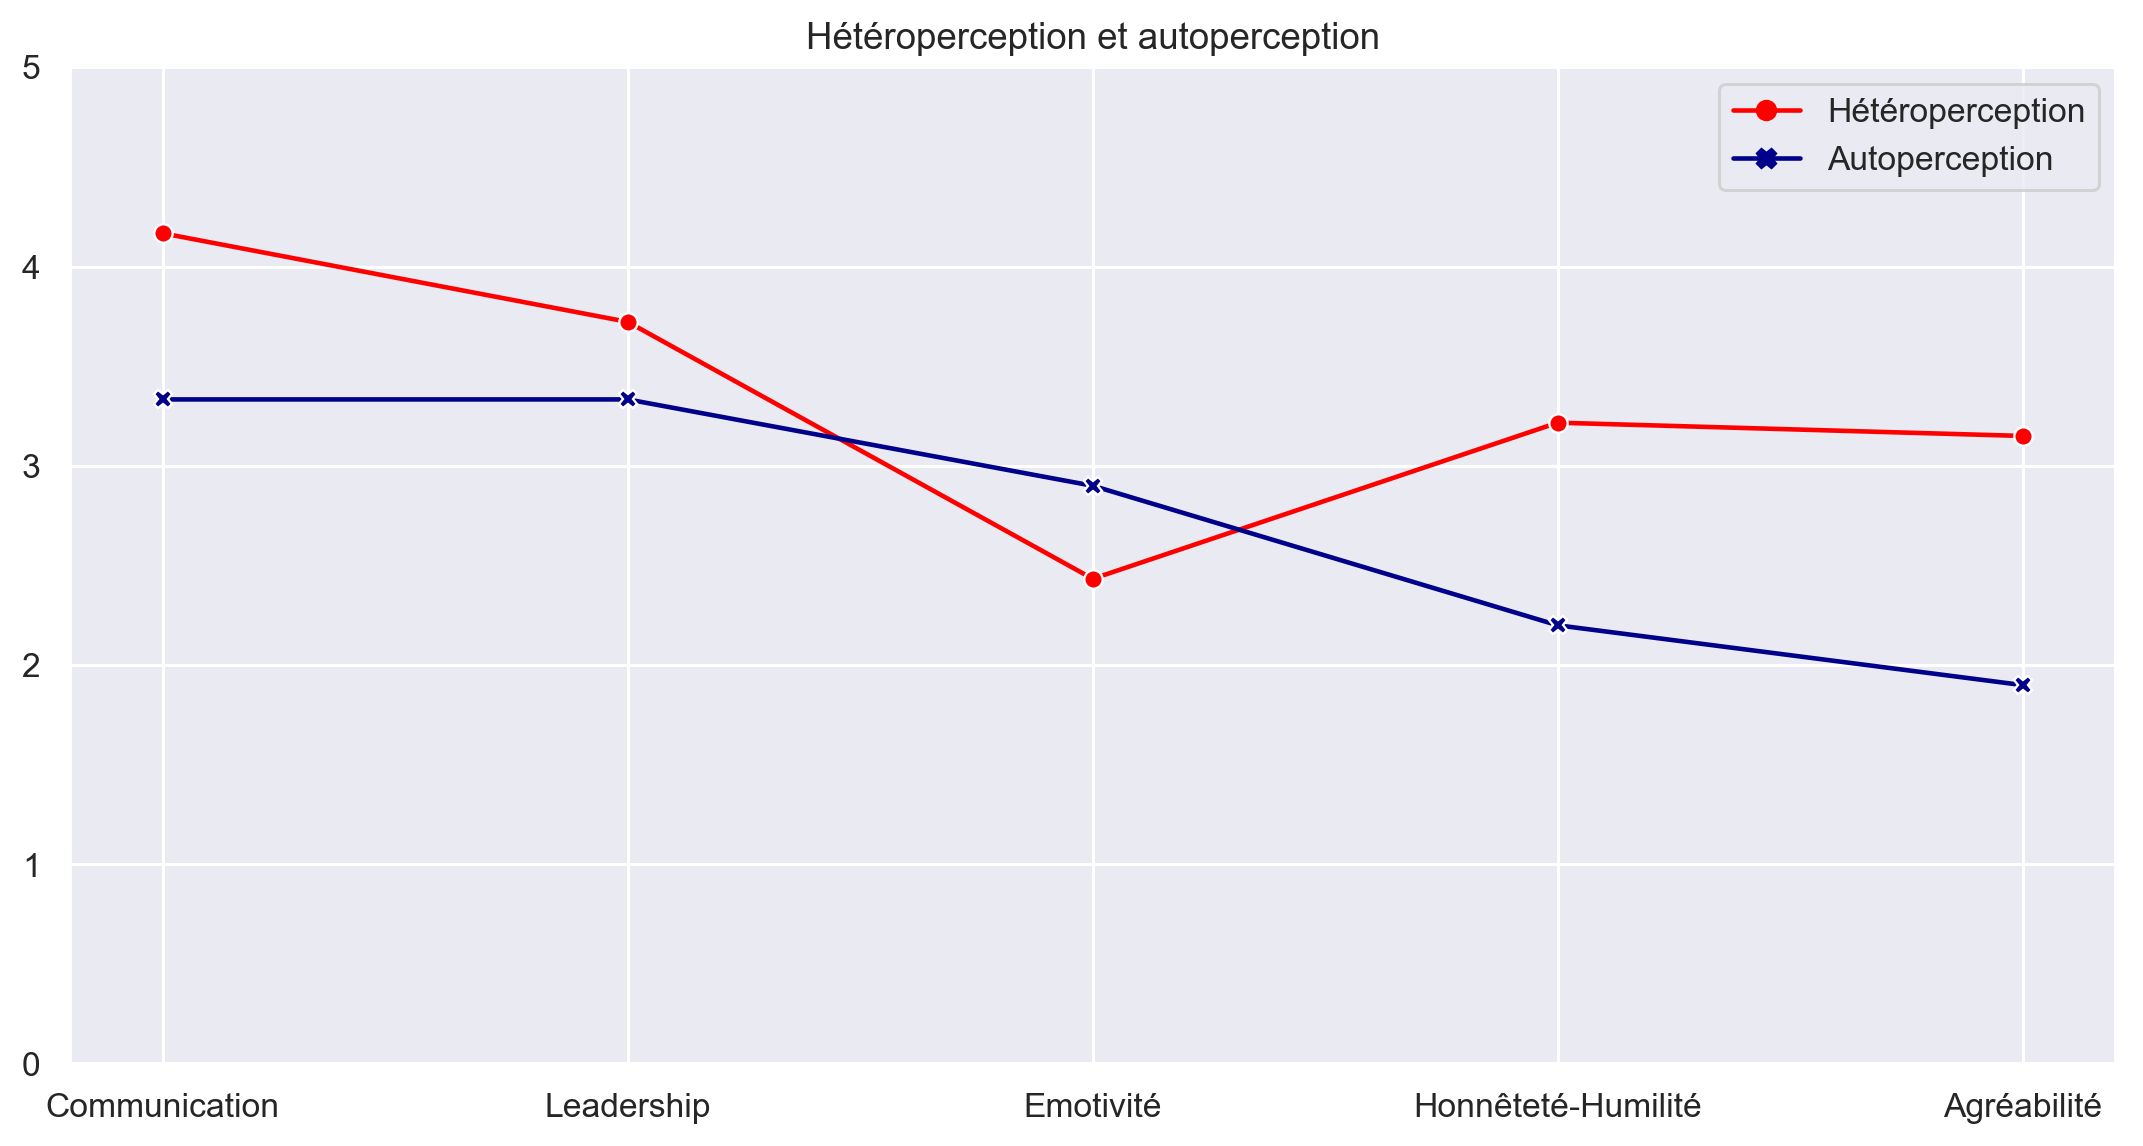
\includegraphics[width=0.95\textwidth]{graph.png}
\end{center}

\textbf{Analyse du graphique}: Le graphique montre... \lipsum[2]

\textbf{Plan de développement personnel}: Fort de ces informations, je peux maintenant... \lipsum[2]

\setlength\parindent{15pt}
\textit{Domaine 1}: la question \codeword{Agr15r} m'a fait comprendre... \lipsum[2]

\textit{Domaine 2}: en faisant référence à \weblink{hexaco.org}... \lipsum[2]

En conclusion... \lipsum[2]

\textit{Lien du questionnaire : }\url{https://ulausannebusiness.eu.qualtrics.com/etcetera}

\end{document} 
